% vim: set nowrap tw=0:
\documentclass[]{llncs}

% \pdfpagewidth=8.5truein{}
% \pdfpageheight=11truein{}

\usepackage{graphicx}
% \renewcommand{\topfraction}{0.99} % be more aggressive about text around floats
% \renewcommand{\floatpagefraction}{0.99}
% \pagestyle{plain} % page numbers

\usepackage{defaultstyle}
\usepackage{localstyle}

\newcommand{\comment}[1]{}%\textsf{#1}}

\title{AppPAL for Android}
\subtitle{Capturing and Checking Mobile App Policies}
% \numberofauthors{2}
\author{Joseph Hallett \and David Aspinall }
\institute{University of Edinburgh}

\begin{document}

\maketitle{}

\begin{abstract}
  % \begin{itemize}
  %   \item \comment{Sentence 1: State the problem}
  Users must judge apps by the information shown to them by the store.
  %   \item \comment{Sentence 2: Why is it an interesting problem}
  Employers rely on employees enforcing company policies correctly on devices at their workplace.
  Some users take time to pick apps with care whilst others do not.
  Users feel frustrated when they realise what data the apps have access to.
  They want greater control over what data they give away but they do not want to spend time reading permissions lists.
  %   \item \comment{Sentence 3: What does my solution achieve}
  We present AppPAL: a policy language to enforce policies about apps.
  AppPAL Policies use statements from third parties and delegation relationships to
  %   \item \comment{Sentence 4: What follows from my solution}
  give us a rigorous and flexible framework for enforcing and comparing and app policies; and the trust relationships surrounding them.
  % \end{itemize}
\end{abstract}

\section{Introduction \comment{1 page}}
\label{sec:introduction}

%\comment{The problem is\ldots}
Finding the right apps can be tricky:
  users need to work out which apps are well written, which are not going to abuse their data, which ones will work in the way they want
  and to find the apps which suit how they want to use their device.
This can be difficult as it isn't obvious how apps use the data each has access to.

App stores give some information about their apps; such as permissions, descriptions of the app and screenshots as well as review scores.
Android apps currently show a confusing list of permissions when they're first installed.
Soon new Android apps will display permissions requests when the app first tries to access sensitive data such as contacts or location information.
Users do not all understand how permissions relate to their device~\cite{Felt:2012hm,Thompson:2013eb}.
Ultimately the decision which apps to use and which permissions to grant must be made by the user.

Not all apps are suitable.
A large amount of \ac{pus} is being propagated for Android devices~\cite{Truong:2014bi,Svajcer:2013tp}.
Employees are increasingly using their own phones for work (bring your own device or BYOD).
An employer may wish to restrict which apps their employees can use.
The IT department may set a policy to prevent information leaks.
Some users worry apps will misuse their personal data;
  such a user avoids apps which can access their location, or address book.
They may apply their own personal security policy when downloading and running apps.

These policies can only be enforced by the users continuously making decisions guided by these policies when prompted about apps.
This is error-prone.
Mistakes can be made.
We believe this can be improved.
An alternative would be to write the policy down and make the computer enforce it.
To implement this we use a logic of authorization.
The policy is written in the logic and enforced by checking the policy is satisfied.

% \begin{figure}
%   \centering
%   \includegraphics[width=0.3\linewidth]{figures/facebook.png}
%   \caption{Security information presented when a user downloads the Facebook app.}
% \label{fig:facebook}
% \end{figure}

%\comment{My contribution is\ldots}
We present AppPAL, an authorization logic for reasoning about apps.
The language is an instantiation of SecPAL~\cite{Becker:2006vh} with constraints and predicates that allow us to decide which apps to run or install.
The language allows us to reason about apps using statements from third parties.
The implementation allows us to enforce the policies on a device.
We can express trust relationships amongst these parties; use constraints to do additional checks.
This lets us enforce deeper and more complex policies than existing tools such as Kirin~\cite{Enck:2009ko}.

Using AppPAL we can say an app is installable:
\begin{lstlisting}
"Alice" says "com.rovio.angrybirds" isInstallable.
\end{lstlisting}
We can delegate decisions to others:
\begin{lstlisting}
"Alice" says "Bob" can-say 0 App isCool.
\end{lstlisting}
We can run analysis tools, and solve constraints:
\begin{lstlisting}
"Claire" says App isMalware
  if App isAnApp
  where
    virusScanner(App) = true.
\end{lstlisting}
Constraints allow up to express facts that are true at some times but not others:
\begin{lstlisting}
"Emma" says "com.facebook.katana" isRunnable
  where timeOfDay() > 1700.
\end{lstlisting}

Specifically we have:
\begin{itemize}
  \item
    Described a scenario where an employer has a policy they want to enforce for their employees~(\autoref{sec:problem}.)
    We show how the trust relationships in a system can be difficult to see;
      and how AppPAL makes the trust between users explicit.
  \item
    Shown how the employer's policy could be implemented using AppPAL~(\autoref{sec:idea}) and installed on Alice's phone.
    We have described what AppPAL would check for an app to meet this policy and how these statements might be collected.

  \item Implemented the AppPAL language on Android and the JVM.
    We show how the language can describe properties of Android apps and Android security poilicies (\autoref{ssec:language}),
      how we evaluate it (\autoref{ssec:eval}),
      and some idiomatic policies (\autoref{ssec:idioms}).

  \item When things go wrong we also need to attribute blame.
    Authorization logic can help make trust relationships explicit.
    We show a recent example of a broken trust relationship (\autoref{ssec:language})
    and how our authorization logic makes explicit where the breach of trust is.

\end{itemize}

\section{Enforcing a policy at work}
\label{sec:problem}

An employee \emph{Alice} works for her \emph{em\/}ployer \emph{Emma}.
Emma allows Alice to use her personal phone as a work phone, but she has some specific concerns.
\begin{itemize}
  \item Alice shouldn't run any apps that can track her movements.
    The testing labs are at a secret location and it mustn't be leaked.
  \item Apps should come from a reputable source, such as the Google Play Store.
  \item Emma uses an \ac{av} program by McAfee.
    It should check all apps before they're installed.
\end{itemize}

To ensure this policy is met Alice promises to follow it.
She might even sign a document promising never to break the rules within the policy.
This is error-prone though---what if she makes a mistake or misses an app that breaks her policy?
Emma's policy could be implemented using existing tools.
The enterprise tool \emph{Google's Device Policy for Android}\footnote{\url{https://play.google.com/store/apps/details?id=com.google.android.apps.enterprise.dmagent}}
could configure Alice's device to disallow apps from outside the Google Play Store (and soon in the newest version of Android let Emma set the permissions of each app on an app by app basis).
Various tools such as AppGuard~\cite{Backes:2012vm}, Dr.~Android~\&~Mr.~Hide~\cite{Jeon:2012ki} or AppFence~\cite{Hornyack:2011wq} can control the permissions or data an app can get.
These could be used to used to ensure no location data is ever obtained.
Alternately other tools like Kirin~\cite{Enck:2009ko}, Flowdroid~\cite{Fritz:2013vi} or DroidSafe~\cite{Gordon:2015et} could check that the locations are ever leaked to the web.
Various anti-virus programs are available for Android---one could be installed on Alice's phone checking against McAfee's signatures.

Whilst we could implement Emma's policy using existing tools, it is a clumsy solution.
They are not flexible: If Emma changes her policy or Alice changes jobs she needs to recheck and then to alter and remove the software on her phone accordingly.
It isn't clear what an app must do to be run, or what checks have been done if it already running on the phone.
The relationship between Alice (the user), Emma (the policy setter) and the tools Emma trusts to implement her policy isn't immediately apparent.

What happens when Alice goes home?
Emma shouldn't be able to overly control what Alice does in her private life.
Alice might not be allowed to use location tracking apps at work, but at home she might want to (to meet friends, track jogging routes or find restaurants for example).
Some mobile OSs allow app permissions to be enabled and disable at run time.
Can we enforce different policies at different times or locations?

Our research looks at the problem of picking software.
Given there are some apps you want to install and run and others you do not want to, at least some of the time:
  how can you express your preferences in such a way that they can be enforced automatically?
How can we translate policy documents from natural language into a machine checkable form?
Furthermore how can we show the trust relationships used to make these decisions clearly and precisely?

\begin{figure}
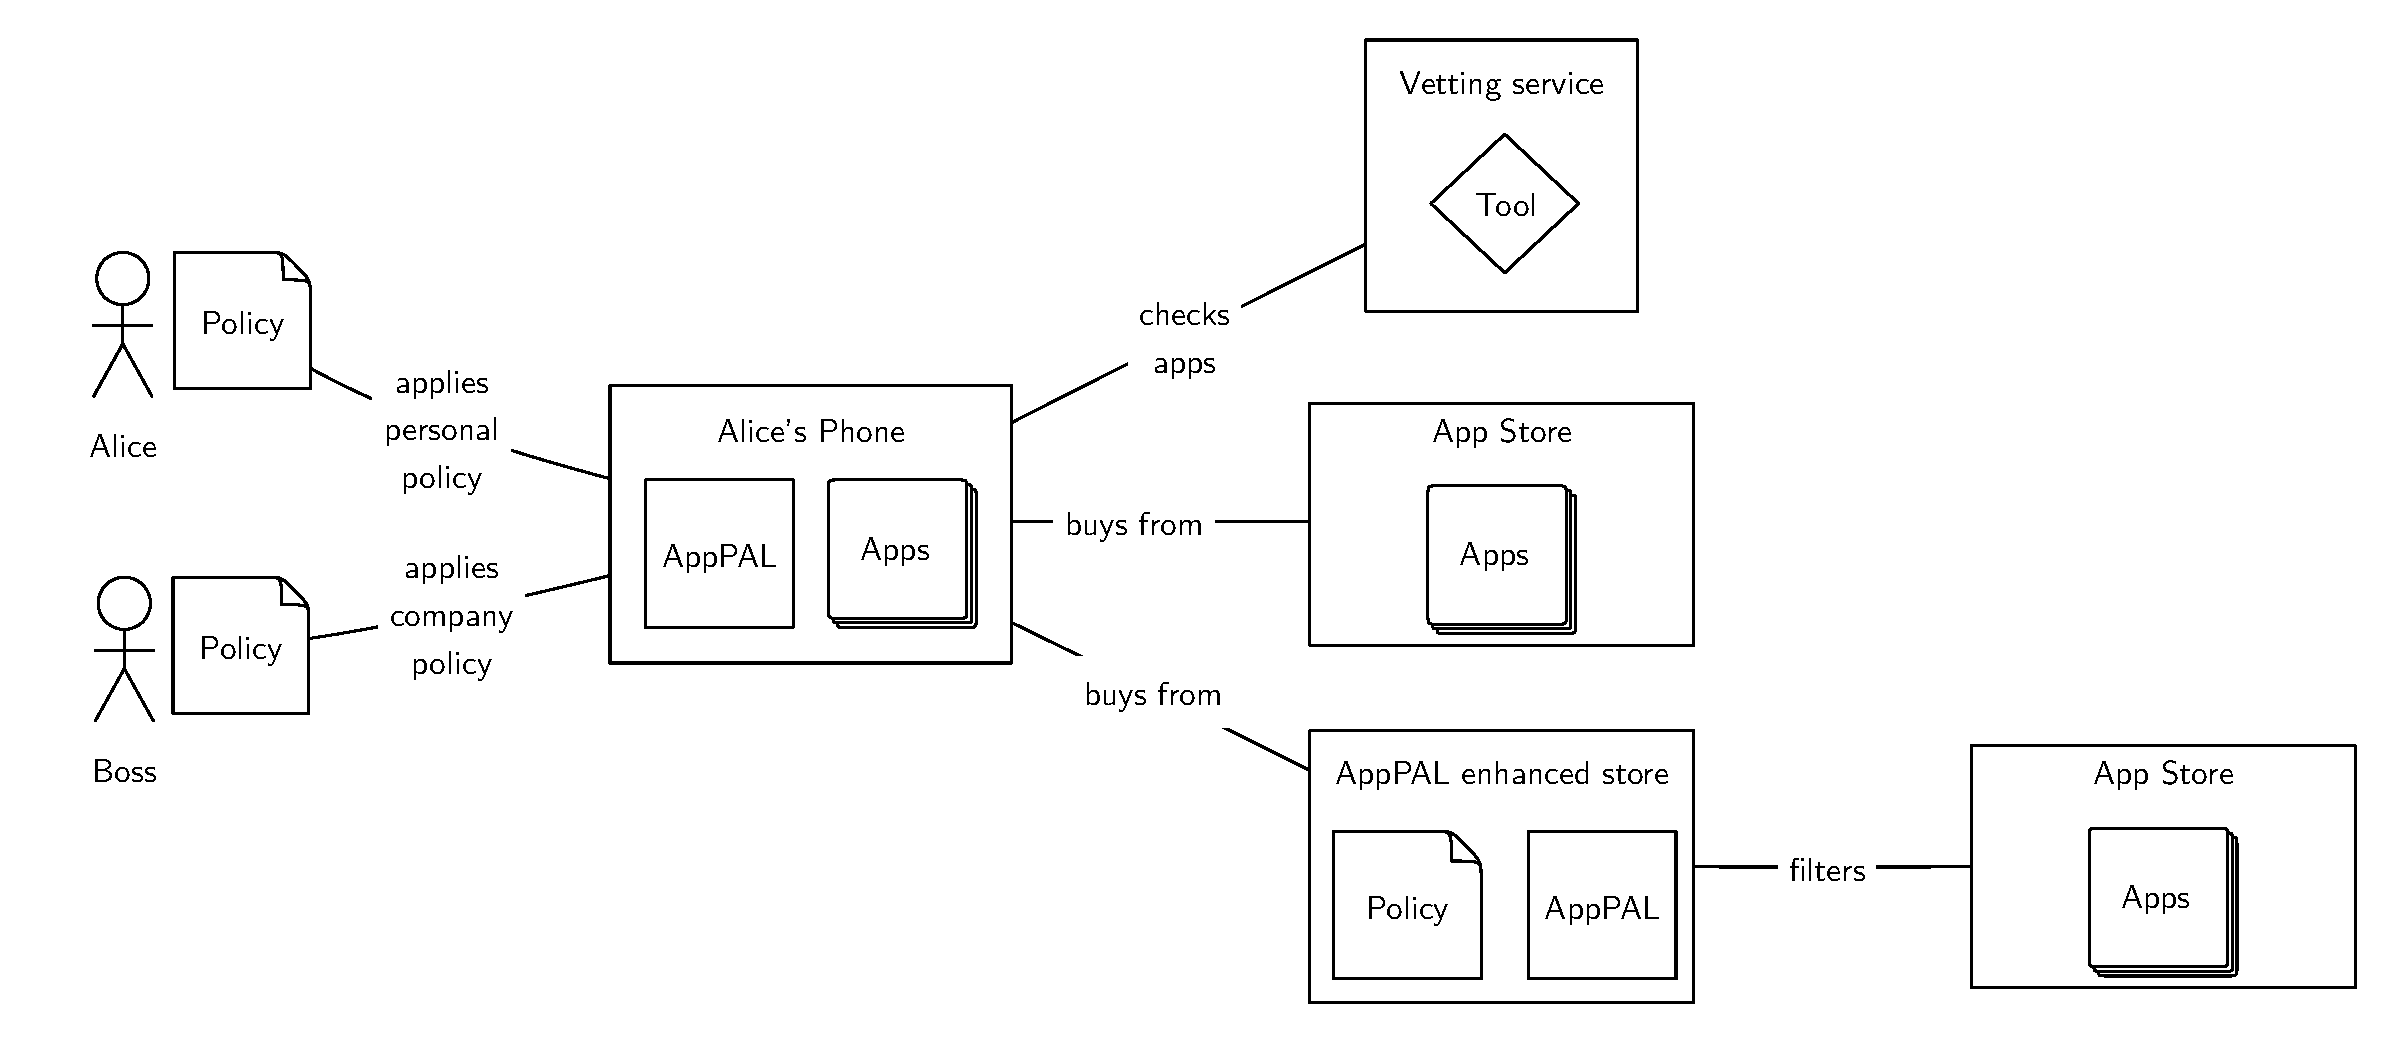
\includegraphics{figures/overview.eps}
\caption{Ecosystem of devices and stores with AppPAL.}
\label{fig:ecosystem}
\end{figure}

We propose a change to the ecosystem, shown in \autoref{fig:ecosystem}.
People have policies which are enforced by AppPAL on their devices.
The device can make use of vetting services which run tools to infer complex properties about apps.
Users can buy from stores which ensure the only apps they see are the apps which meet their policies.

\section{Expressing policies in AppPAL}
\label{sec:idea}

In \autoref{sec:problem} Alice and Emma's had policies they wanted to enforce but no means to do so.
Instead of using several different tools to enforce Emma's policy disjointedly, we use an authorization logic.
In \autoref{lst:corporate} we give an AppPAL policy implementing Emma's app concerns on Alice's phone.
% A pictorial representation, is given in \autoref{fig:emmas_policy}; color splits statements by each speaker.

% \begin{figure}
%   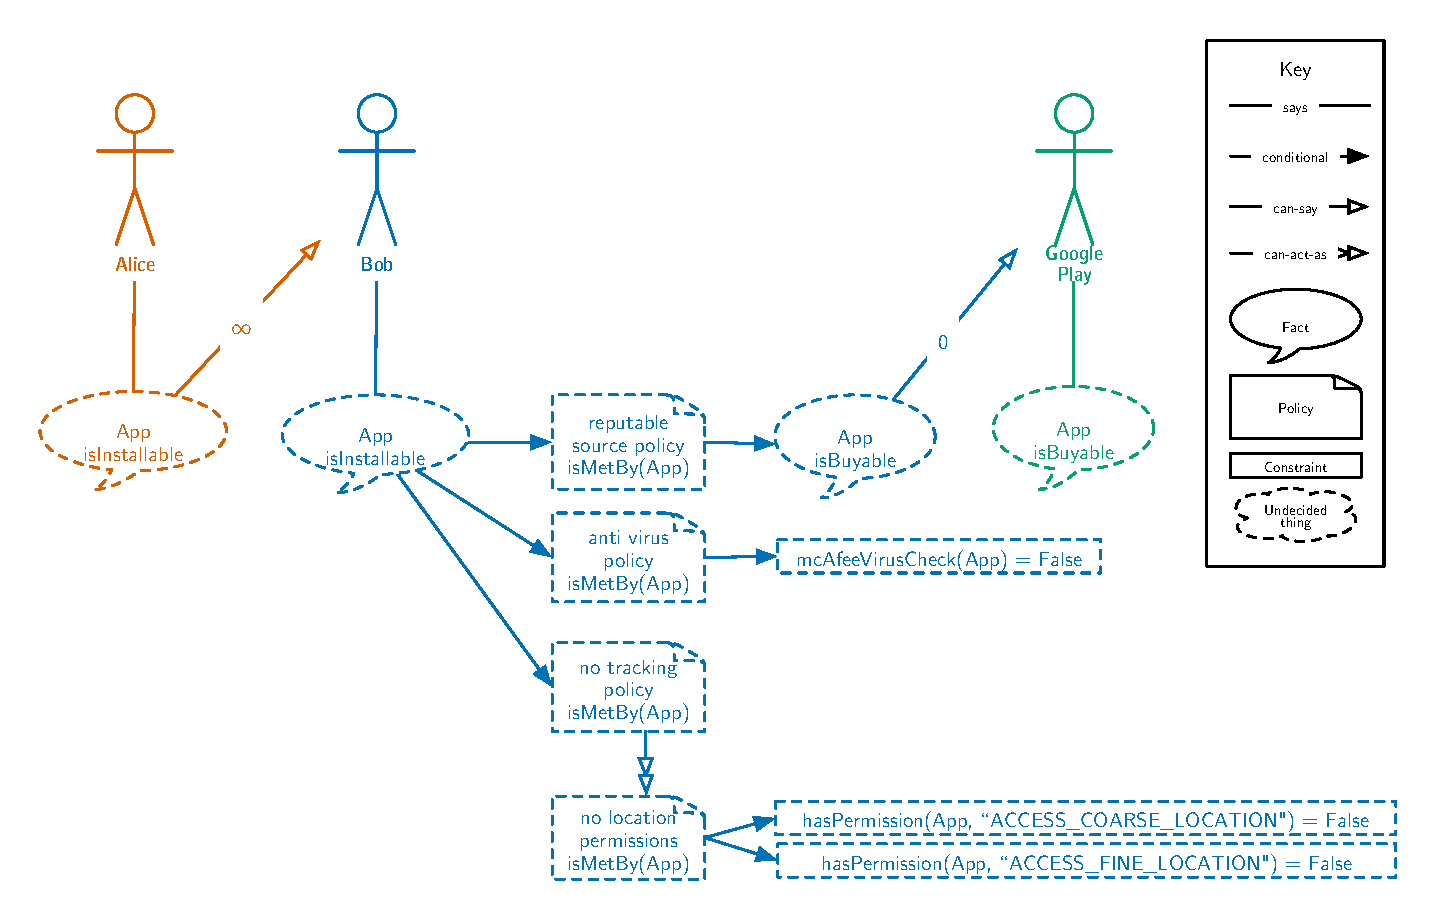
\includegraphics{figures/bob-policy.eps}
%   \caption{Pictorial representation of Alice's app install policy.}
% \label{fig:emmas_policy}
% \end{figure}

AppPAL is an instantiation of SecPAL~\cite{Becker:2006vh} for describing app policies.
SecPAL is a logic of authorization for access control decisions in distributed systems.
It has a clear and readable syntax, as well as rich mechanisms for delegation and constraints.
SecPAL has already been used as a basis for other policy languages in areas such as privacy preferences~\cite{Becker:2009ula} and data-sharing~\cite{Aziz:2011vt}.
We present AppPAL as a new version of SecPAL, targeting apps on mobile devices.

\begin{figure}
  \begin{minipage}[t]{0.5\textwidth}
    \begin{lstlisting}[numbers=left,
                       escapeinside={@}{@}]
"alice" says "emma" can-say inf
  App isRunnable. @\label{lst:corporate_1}@

"emma" says App isRunnable @\label{lst:corporate_2}@
  if "no-tracking-policy" isMetBy(App),
     "reputable-policy" isMetBy(App),
     "anti-virus-policy" isMetBy(App).

"emma" says
  "reputable-policy" isMetBy(App) @\label{lst:corporate_3}@
      if App isReputable.

"emma" says "google-play" can-say 0
  App isReputable. @\label{lst:corporate_4}@
    \end{lstlisting}
  \end{minipage}\begin{minipage}[t]{0.5\textwidth}
    \begin{lstlisting}[numbers=left,
                       escapeinside={@}{@},
                       firstnumber=14]
"emma" says "anti-virus-policy" isMetBy(App) @\label{lst:corporate_5}@
  if App isAnApp
  where
    mcAfeeVirusCheck(App) = false.

"emma" says "no-location-permissions"
  can-act-as "no-tracking-policy". @\label{lst:corporate_6}@

"emma" says
  "no-location-permissions" isMetBy(App) @\label{lst:corporate_7}@
    if App isAnApp
    where
      hasPermission(App, "LOCATION")=false.
\end{lstlisting}
\end{minipage}
\caption{AppPAL policy implementing Emma's security requirements}
\label{lst:corporate}
\end{figure}

In \autoref{lst:corporate_1} Alice gives Emma the ability to specify whether an \code{App} (a variable) \code{isRunnable} (a predicate).
She allows her to delegate the decision further if she chooses (\code{can-say inf}).
Next in \autoref{lst:corporate_2} Emma specifies her concerns as policies to be met (the \code{isMetBy()} predicate that takes an app as its argument).
If Emma can be convinced all these policies are met then he will say the \code{App isRunnable}.
In \autoref{lst:corporate_3} and \autoref{lst:corporate_4} Emma specifies that an app meets the \code{reputable-policy} if the \code{App isReputable};
  with \code{"google-play"} specified as the decider of what is buyable or not.
This time Google is not allowed to delegate the decision further (\code{can-say  0}).
In other words Google is not allowed to specify Amazon as a supplier of apps as well.
Google must say what is buyable directly for Emma to accept it.
Emma specifies the \code{"anti-virus-policy"} in \autoref{lst:corporate_5}.
Here we use a constraint.
When checking the policy the \code{mcAfeeVirusCheck} should be run on the \code{App}.
Only if this returns \code{false} will the policy be met.
To specify the \code{"no-tracking-policy"} Emma says that the \code{"no-location-permissions"} rules implement the \code{"no-tracking-policy"} (\autoref{lst:corporate_6}).
Emma specifies this in \autoref{lst:corporate_7} by checking the app is missing two permissions.

Say Alice wants to install a new app (\code{com.facebook.katana}) on her phone.
To meet Emma's policy the AppPAL policy checker needs to collect statements to show the app meets the \code{isRunnable} predicate.
Specifically it needs:
\begin{itemize}
  \item\code{"emma" says "com.facebook.katana" isAnApp.}
    A simple typing statement that can be generated for all apps as they are encountered.
    This helps keep the number of  assertions in the policy low aiding readability.
  \item\code{"google-play" says "com.facebook.katana" isReputable.}
    Required to convince Emma the app came from a reputable source.
    It should be able to obtain this statement from the Play store as the app is available there.
  \item\code{"emma" says "anti-virus-policy" isMetBy("com.facebook.katana").}
    She can obtain this by running the \ac{av} program on her app.
  \item\code{"emma" says "no-locations-permissions" isMetBy("com.facebook.katana").}
    Needed to show the App meets Emma's no-tracking-policy.
    Emma will say this if after examining the app the location permissions are missing.
\end{itemize}
These last two statements require the checker to do some extra checks to satisfy the constraints.
To get the third statement it must run the \ac{av} program on her app and check the result.
The results from the \ac{av} program may change with time as it's signatures are updated;
  so the checker must re-run this check every time it wants to obtain the statement connected to the constraint.
For the forth statement the checker needs to check the permissions of the app.
It could do this by looking in the \texttt{MANIFEST.xml} inside the app itself.

In this scenario we have imagined Alice wanting to check the apps as she installs them.
Alternatively we could imagine Emma wanting a personalised app store where all apps sold meet her policy.
With AppPAL this can be implemented by taking an existing store and selectively offering only the apps which will meet the user's policy.
This gives us a \emph{filtered store}.
From an existing set of apps we produce a personalised store that meets a pre-defined policy.

\section{AppPAL}
\label{sec:details}

AppPAL is implemented as a library for Android and Java.
The parser is implemented using ANTLR4.
Code and build instructions are available from Github\footnote{\url{https://github.com/bogwonch/libAppPAL}}.

\subsection{The Language}
\label{ssec:language}

The structure of an AppPAL assertion can be seen in \autoref{fig:assertion}.

\begin{figure}
  \centering
  \begin{equation*}\small
    \begin{array}{r l}
      \overbrace{\text{\ttfamily "user"}}^{\text{speaker}} &
      \text{\ttfamily says }\overbrace{\overbrace{\text{\ttfamily App }}^{\text{subject}}\overbrace{\text{\ttfamily isRunnable}}^{\text{predicate}}}^{\text{fact}} \\
      & \overbrace{\text{\ttfamily if App isFree}}^{\text{condition}} \\
      & \overbrace{\text{\ttfamily where hasPermission(App, "INTERNET") = true}}^{\text{constraint}}.
    \end{array}
  \end{equation*}
  \caption{Structure of an AppPAL assertion.}
\label{fig:assertion}
\end{figure}

In the Becker~\etal's paper~\cite{Becker:2006vh} they leave the choice of predicates, and constraints for their SecPAL open.
With AppPAL we make explicit our predicates and how they relate to Android.
Some of these predicates require arguments.
We add a light typing system to help ensure these predicates have the correct arguments.

Specifically we define the following predicates:
\begin{description}
  \item[\texttt{App isRunnable}]
    Used to indicate that an App meets the install policy for the device.
    Showing an app satisfies this predicate is usually the goal of evaluating AppPAL.

  \item[\texttt{App isAnApp}, \texttt{Policy isAPolicy}\ldots]
    Expresses a simple typing relations.
    AppPAL, and SecPAL, have a safety condition that all variable mentioned in the fact, are also mentioned in the condition body (as is the case for Datalog and other logic languages).
    These typing relations allow an appeal to ground facts to be made so the safety condition is satisfied.
    This typically is necessary when an assertion has a constraint but no body conditions: we add the trivial typing statement to the body to ensure the assertion is accepted by AppPAL.

  \item[\texttt{Policy isMetBy(App)}]
    Policies let you split app behaviour into sub-policies.
    For example in \autoref{sec:idea} we showed how Emma's installation policy could be written using three \texttt{isMetBy} statements.
    Splitting policies allows greater control of how each one is checked.
    We can delegate checking a policy to an expert using the \code{can-say} statement.
    We can specify more detailed checks using the \code{can-act-as} statements.

  \item[\texttt{Policy shownIsMetBy(Evidence, App)}]
    A variant of the \texttt{isMetBy} statement that allows some evidence (a proof) to be given that shows the policy is met.
\end{description}

Splitting the decision about whether an app is runnable into a series of policies that must be met gives us flexibility in how the decision is made.
It allows us to describe multiple means of making the same decision, and provide backup routes when one means fails.
Some static analysis tools are not quick to run.
Even taking minutes to run a battery draining analysis can be undesirable.
If a user wants to download an app quickly they may not be willing to wait to check that a policy is met.

Consider the \emph{no-tracking-policy} from earlier.
In Bob's policy we checked this by checking the permissions of the app.
If the app couldn't get access to the GPS sensors (using the permissions) then it met this policy.
Some apps may want to access this data, but may not leak it.
We could use a taint analysis tool to detect this (e.g.~Taintdroid~\cite{Fritz:2013vi}).
Our policy now becomes:

\begin{lstlisting}
"bob" says "no-locations-permissions"
  can-act-as "no-tracking-policy".

"bob" says "no-locations-permissions" isMetBy(App)
  if App isAnApp
  where
    hasPermission(App, "ACCESS_FINE_LOCATION") = false,
    hasPermission(App, "ACCESS_COARSE_LOCATION") = false.

"bob" says "location-taint-analysis"
  can-act-as "no-tracking-policy".

"bob" says "location-taint-analysis" isMetBy(App)
  if App isAnApp
  where
    taintDroidCheckLeak(App, "Location", "Internet") = false.
\end{lstlisting}

Sometimes we might want to use location data.
For instance Bob might want to check that Alice is at her office.
Bob might track Alice using a location tracking app.
Provided the app only talks to Bob, and it uses SSL correctly (which Mallodroid can check for~\cite{Fahl:2012dj}) he is happy to relax the policy.

\begin{lstlisting}
"bob" says "relaxed-no-tracking-policy" canActAs "no-tracking-policy".
"bob" says "relaxed-no-tracking-policy" isMetBy(App)
  if App hasCategory("tracking")
  where
    mallodroidSSLCheck(App) = false,
    connections(App) = "[https://bob.com]".
\end{lstlisting}

This gives us four different ways of satisfying the \emph{no-tracking-policy}:
  with permissions,
  with taint analysis,
  with a relaxed version of the policy,
  or by Bob directly saying the app meets it.
When we come to check the policy if any of these ways give us a positive result we can can stop our search.

AppPAL also helps attribute blame when things go wrong.
By modelling the trust relationships in systems we can work out precisely where mistakes were made.
A recent example demonstrating this is \textsc{CVE-2015-2077}.
Lenovo was found to be shipping laptops with the \emph{Superfish} malware pre-installed.
Lenovo had also installed an \ac{av} package on their laptops; this \ac{av} did recognise Superfish as malware.
Unfortunately they had configured it to ignore Superfish.
The malware was an ad framework designed to show users products similar to those they viewed on the web.
Unfortunately it did so by man-in-the-middling all SSL traffic using a shared private key.

From a user's perspective there was a delegation of trust to Lenovo to detect malware.
Lenovo then delegated further to McAfee to supply the antivirus checking; but left an exception that they would allow Superfish.
A user might wonder where the breach of trust occurred and who is to blame?
Is it the \ac{av} failing to spot the malware?
Has someone else configured the software incorrectly?
How should they fix the problem?

If we write this in the AppPAL policy language the cause of the breach of trust becomes apparent; as does the fix.
\begin{lstlisting}[numbers=left, escapeinside={@}{@}, label={lst:lenovo}]
"user" says "lenovo" can-say inf File isSafe. @\label{lst:lenovo_trust}@
"lenovo" says "mcafee" can-say inf File isSafe.
"lenovo" says "C:\System\superfish" isSafe. @\label{lst:lenovo_unsafe}@
\end{lstlisting}
The fault lies with \autoref{lst:lenovo_unsafe}.
Lenovo has caused the problem (they \emph{said} it was safe).
The fix is to revoke this statement, or to revoke \autoref{lst:lenovo_trust} and find a different \ac{av} supplier.

\subsection{Evaluation}
\label{ssec:eval}

To evaluate AppPAL we implement the SecPAL evaluation rules shown in \autoref{fig:rules}.
We do not use the DatalogC~\cite{Li:2003ix}~based translation and evaluation algorithm suggested by Becker~\etal.
Rather we implement the rules directly in Java.
Pseudo-code is given in \autoref{fig:pseudocode}.
Like Becker~\etal we make use of an assertion context to store known statements.
We also store intermediate results to avoid re-computation.
On a mobile device memory is at a premium.
We would like to keep the context as small as possible.
For some assertions (like \code{isAnApp}) we derive them by checking the arguments at evaluation time.

\begin{figure}
\[\footnotesize
% AC, D ⊧ A says B can-act-as C   AC, D ⊧ A says C verbphrase
% ----------------------------------------------------------- (can-act-as)
%                 AC, D ⊧ A says B verbphrase
\infer[\text{\tiny can-act-as}]{
  AC, D \models \text{\tt A says B verbphrase}}{%
  AC, D \models \text{\tt A says B can-act-as C} & %
  AC, D \models \text{\tt A says C verbphrase}}
\]
\[\footnotesize
% AC, ∞ ⊧ A says B can-say D fact   AC, D ⊧ B says fact
% ----------------------------------------------------- (can-say)
%                   AC, ∞ ⊧ A says fact
\infer[\text{\tiny can-say}]{
  AC, \infty \models \text{\tt A says fact}}{%
  AC, \infty \models \text{\tt A say B can-say $D$ fact} & %
  AC, D \models \text{\tt B says fact}}
\]
\[\footnotesize
% (A says fact if fact₁, …, factₖ, c) ∈ AC
% AC, D ⊧ A says factᵢθ  ∀i ∈ {1…k}    ⊧cθ    vars(factθ) = ∅
% ----------------------------------------------------------- (cond)
%                    AC, D ⊧ A says factθ
\infer[\text{\tiny cond}]{
  AC, D \models \text{\tt A says fact$\theta$}}{
  \begin{array}{c}
    (\text{\tt A says fact if fact$_1$, \ldots, fact$_k$ where c}) \in AC \\
    \forall i \in 1\cdots k.\;AC, D \models \text{\tt A says fact$_i\theta$}
  \end{array} &
  \models \mathtt{c}\theta &
  \text{\sl vars}(\text{\tt fact$\theta$}) = \emptyset}
\]
\caption{AppPAL's evaluation rules.}
\label{fig:rules}
\end{figure}

This gives us greater control of the evaluation and how the assertion context is created.
For example, when checking the \code{isAnApp} predicate;
  we can fetch the assertion that the subject is an app based on the app in question.
Similarly when we use a statement from \emph{Emma} that \emph{Google-Play can-say} whether an app is buyable;
  it is sensible to go fetch from the store whether the app is saleable and make Google say it then and there.

In SecPAL there is no type.
All entities are either constants (implemented as strings) or variables.
There is no differentiation made between a \emph{voiced} constant (who says assertions),
and a \emph{subject} (the subject of a verb-phrase, or predicate argument).
In AppPAL the subjects are usually apps or policies.
Apps do not utter facts;
  so there is no need to check them as potential speakers of \emph{can-say} statements.
Similarly if a constant never appears as a subject of a statement, as most speakers do not,
  there is no need to check it as a possible subject for a \emph{can-act-as} statement.
We pre-process the assertion context to find \emph{voiced} and \emph{subject} constants.
This means we need to search less constants when attempting to replace a variable, speeding evaluation.

\begin{figure}
\begin{minipage}[b]{0.5\linewidth}
\begin{lstlisting}[language=Ruby, basicstyle=\ttfamily\scriptsize, keywordstyle=\scriptsize\slshape, columns=flexible]
# ac, d |-? q (using previous-results table rt)
def evaluate(ac, rt, q, d)
  return rt[q, d] if rt.contains q, d
  p = cond(ac, rt, q, d)
  return (Proven, rt.update q, d, p) if p.isValid
  p = canSay_CanActAs(ac, rt, q, d)
  return (Proven, rt.update q, d, p) if p.isValid
  return (Failure, rt.update q, d, Failure)

# Try can-say and can-act-as
def canSay_CanActAs(ac, rt, q, d)
  ac.constants.each do |c|
    if c.is_a :subject
      p = canActAs ac, rt, q, d
      return Proven if p.isValid
    elsif c.is_a :speaker
      p = canSay ac, rt, q d
      return Proven if p.isValid
  return Failure
\end{lstlisting}
\end{minipage}
\begin{minipage}[b]{0.5\linewidth}
\begin{lstlisting}[language=Ruby, basicstyle=\ttfamily\scriptsize, keywordstyle=\scriptsize\slshape, columns=flexible]
# Try cond rule
def cond(ac, rt, q, d)
  ac.add q.fetch if q.isFetchable
  ac.assertions.each do |a|
    if (u = q.unify a.consequent) &&
       (a = u.substitution a).variables == none
      return checkConditions ac, rt, a, d
  return Failure

# Evaluate the antecedents
def checkConditions(ac, rt, a, d)
  getVarSubstitutions(a,ac.constants).each do |s|
    sa = s.substitute a
    if sa.antecedents.all
        { |a| evaluate(ac, rt, a, d).isValid }
      p = evaluateC sa.constraint
      return Proven if p.isValid
  return Failure
\end{lstlisting}
\end{minipage}
\caption{Partial-pseudocode for AppPAL evaluation.}
\label{fig:pseudocode}
\end{figure}

\subsection{Policy Examples}
\label{ssec:idioms}

When writing policies some schemes often come up.
We give examples of policies and queries and show how they can be implemented in AppPAL.

\begin{description}
  \item[Policies for home and work]
    In \autoref{sec:introduction} we said Alice might like to have separate rules for home and work.
    Emma may insist that her policies come into effect whenever Alice is at work, but is okay with Alice breaking them after 5~pm or when she isn't at work.
    To implement this we add rules that use constraints to decide whether an app should be run.
    Alice already has the Emma's work policy as the default.
    Now she just needs to add an exception to the rule.
    \begin{lstlisting}
"alice" says App isRunnable
  if "home-policy" isMetBy(App)
  where TimeOfDay() > 17.00.

"alice" says App isRunnable
  if "home-policy" isMetBy(App)
  where At("work") = false.
    \end{lstlisting}

  \item[App white-listing by an IT department]
    Inside Emma's company employees in the IT department may white-list certain apps as runnable.
    Emma delegates to them to decide if an app is runnable.
    \begin{lstlisting}
"emma" says "it-department" can-say 0 App isRunnable.
    \end{lstlisting}
    Charlie and Diveena work in the IT department.
    When they have checked an app they say it is runnable.
    \begin{lstlisting}
"emma" says "charlie" can-act-as "it-department".
"emma" says "diveena" can-act-as "it-department".

"charlie" says "com.facebook.katana" isRunnable.
"diveena" says "org.thoughtcrime.securesms" isRunnable.
    \end{lstlisting}

  \item[Overpriviliged applications]
    Alice is particularly worried about apps stealing her data.
    She knows that certain apps need certain permissions.
    For example a photography app needs access to the camera.
    She checks each app's permissions carefully for things that seem unusual.

    Alice's policy can be implemented by checking the permissions of the app, using constraints.
    \begin{lstlisting}
"alice" says App isRunnable
   if "permissions-policy" isMetBy(App).
"alice" says "permissions-policy" isMetBy(App)
   if App isAnApp
   where
      category(App, "Photography"),
      hasPermission(App, "LOCATION") = false,
      hasPermission(App, "CAMERA") = true.
    \end{lstlisting}

    Discovering the \emph{normal} permissions for an app can be done by mining large stores of apps, or apps a user has previously installed.
    Alternately tools like Stowaway~\cite{Felt:2011kj} could be integrated to check apps.

  \item[Digital Evidence]
    In \autoref{ssec:language} we described how digital evidence could be used to decide if policies are met.
    Suppose a digital evidence generating tool, such as \emph{Evicheck}, can be used to check a policy.
    For example that no audio can be recorded without the users consent~\cite{Seghir:2014uq}.
    Using this tool someone generates a proof certificate that this property is met.
    This might be the developer of the app, a third party certification service, or someone else;
      when we check the proof we will discover if it is valid or not.
    \begin{lstlisting}
"alice" says Anyone can-say 0
  "recording-consent" shownIsMetBy(Evidence, App).

"skb" says "recording-consent"
  shownIsMetBy("evicheck://evidence123", App).

"alice" says "recording-consent" isMetBy(App)
  if "recording-consent" shownIsMetBy(Evidence, App)
  where
    evicheckCheckEvidence(Evidence, App) = true.
    \end{lstlisting}
    In the example here Alice allows anyone to present her with evidence for her policy.
    A \ac{skb} offers some evidence, and Alice accepts it as if it checks out.
\end{description}

\section{Related work}

Authorization logics have been successfuly used to enforce policies in several other domains.
The earliest such logic, PolicyMaker~\cite{Blaze:dj}, was general, if undecidable.
Logics that followed like KeyNote~\cite{Blaze:1999fa} and SPKI/SDSI~\cite{Ellison:1999ui} looked at public key infrastructure.
The RT-languages~\cite{Li:2002if,Li:2003ix,Li:2003to} were designed for credential management.
Cassandra~\cite{Becker:2004fi} was used to model trust relationships in the british national health service.

SELinux is used to describe policies for Linux processes, and for access control (on top of the Linux discretionary controls).
It was ported to Android~\cite{Smalley:2013vl} and is used in the implementation of the permissions system.
Google also offer the \emph{Device Policy for Android} app.
This lets businesses to configure company owned devices to be trackable, remote lockable, set passwords and sync with their servers.
It cannot be used to describe policies about apps, or describe trust relationships, however.

The SecPAL language was initially used for access control in distributed systems.
We picked SecPAL as the basis for AppPAL because it was readable, extensible, and seemed to be a good fit for the problem we were trying to solve~\cite{Hallett:2014un}.
It has already been used to describe data usage policies~\cite{Aziz:2011vt} and inside Grid data systems~\cite{Humphrey:2007wc}.
Other work on SecPAL has added various features such as existential quantification~\cite{Becker:2009vt} and ultimately becoming the DKAL family of policy languages~\cite{Gurevich:2008fz,Gurevich:Qo5E3M3}.
Gruevich and Neeman showed that SecPAL was a subset of DKAL (minus the \emph{can-act-as} statement).
DKAL also contains more modalities than \emph{says}, which lets policies describe actions principals carry out rather than just their oppinions.
For example in AppPAL a user might \emph{say} an app is installable if they would install it (\code{"user" says App isInstallable})
In DKAL they can describe the conditions that would force them to install it (\code{"user" installs App}).
The distinction is that in AppPAL whilst the user thinks the app could be installed we do not know for sure whether the user has installed it.
With the DKAL we can guarantee that the action was completed.

One tool, Kirin~\cite{Enck:2009ko}, also created a policy language and tool for enforcing app installation policies.
Kirin's policies were concerned with preventing malware.
Policy authors could specify combinations of permissions that should not appear together.
For example an author might wish to stop malware sending premium rate text messages.
To might implement this by restricting an app having both the \texttt{SEND\_SMS} and \texttt{WRITE\_SMS} permissions (\autoref{fig:kirin}).
Using this approach they found vulnerabilities in Android, but were ultimately limited by being restricted to permissions and broadcast events.
\begin{figure}
\begin{lstlisting}
restrict permission [SEND_SMS] and permission [WRITE_SMS]
\end{lstlisting}
\begin{lstlisting}
"user" says "no-write-send-sms" isMetBy(App)
  where hasPermission(App, "SEND_SMS") = false.
"user" says "no-write-send-sms" isMetBy(App)
  where hasPermission(App, "WRITE_SMS") = false.
\end{lstlisting}
\caption{Kirin and AppPAL policies for stopping apps monetized by premium rate text messages.}
\label{fig:kirin}
\end{figure}

Whilst this approach is great for malware, it is less suitable for finding \ac{pus}.
The behaviours and permissions \ac{pus} apps display aren't necessarily malicious.
One user may consider apps which need in-app-purchases to play malware, but another may enjoy them.
AppPAL tries to stop these \ac{pus} apps.
Because we can use external checking tools which go further than permissions checks, our policies can be richer.
By allowing delegation relationships we can understand the provenance and trust relationships in these rules.

Work by Lin~\etal looked at modelling users' willingness to grant different kinds of permissions~\cite{Sadeh:2014vq}.
They found four clusters of different users each with different kinds of policies:
  conservatives who do not like granting many permissions,
  advanced users who seem to have more complex policies,
  unconcerned users who'll comfortably grant anything,
  and fence-sitters (about half of all users) who seemed not to have varying opinions.
This suggests that users are applying policies and do care how apps behave.
Lin~\etal speculate that the fence-sitters seemed not to care because of \emph{warning fatigue}.
This suggests a system like AppPAL that can reduce user interaction with permission warnings might be interesting.
Using a policy unconcerned and fence-sitting users could take up more privacy preserving policies without having to change their behavior.
We have created an Android app that can check approximations of Lin~\etal's policies against apps on a users device.
This gives us a demonstration of the power of AppPAL using known policies\footnote{\url{https://github.com/bogwonch/apppal-checker}}.

There has been a great amount of work on developing app analysis tools for Android.
Tools such as Stowaway~\cite{Felt:2011kj} detect overprivileged apps.
TaintDroid~\cite{Enck:2010uw} and FlowDroid~\cite{Fritz:2013vi} can do taint and control flow analysis; sometimes even between app components.
Other tools like QUIRE~\cite{Bugiel:2012ui} can find privilege escalation attacks between entire apps.
ScanDAL~\cite{Kim:2012vt} and SCanDroid~\cite{Fuchs:2009vi} help detect privacy leaks.
Appscopy~\cite{Feng:kPGZr_ja} searches for specific kinds of malware.
Tools like DroidRanger~\cite{Zhou:2012tb} scan app markets for malicious apps.
Many others exist checking and certifying other aspects of app behaviour.

\section{Conclusions and further work \comment{$\frac{1}{2}$ page}}

We have presented AppPAL: an authorization logic for describing app installation policies.
The language is implemented in Java and runs on Android using a custom evaluation algorithm.
This lets us to enforce app installation policies on Android devices.
We have shown how the language can be used to describe an app installation policy;
  and given brief descriptions of how other policies might be described.

Further work is required to tightly integrate AppPAL into Android.
One way to integrate AppPAL on Android would be as a \emph{required checker}: a program that checks all apps before installation.
Google uses this API to check for known malware and jailbreak apps.
We would use AppPAL to check apps meet policies before installation.
Unfortunately the API is protected and it would require the phone to be rooted to run there.
Alternatively AppPAL could be integrated as a service to reconfigure app permissions.
The latest version of Android\footnote{Called \emph{Android M}.} is moving to a more iOS like permissions model where permissions can be granted and revoked at any time.
These will be manually configurable by the user through the settings app.
We can imagine AppPAL working to reconfigure these settings (and set their initial grant or deny states) based on a user's policy, as well as the time of day or the user's location.
A policy could deny pop-up notices while a user is driving for example.

Developing, and testing, policies for users is a key next step.
Here we described a policy being specified by a company boss.
For most end-users writing a policy in a formal language is too much work.
Ad-blocking software works by users subscribing to filter policies written by experts\footnote{EasyList is a popular choice and the default in most ad-blocking software. They offer many different policies for specific use-cases however. \url{https://easylist.adblockplus.org/en/}}.
We can imagine a similar scheme working well for app installation policies.
Users subscribe to different policies by experts (examples could include no tracking apps, nothing with adult content, no spammy in-app-purchase apps).
Optionally they can customize them further.

We should also attempt to learn policies from existing users behavior.
Given app usage data, from a project like Carat~\cite{Oliner:2013ht}, we could identify security conscious users.
If we can infer these users policies we may be able to describe new policies that the less technical users may want.
Given a set of apps one user has already installed, we could learn policies about what their personal installation policy is.
This may help stores show users apps they're more likely to buy, and users apps that already behave as they want.

AppPAL is a powerful language for describing app installation policies.
It gives us a framework for describing and evaluating policies for Android apps.
The work provides new ways for users to enforce their own rules about how apps should behave.
Users policies can be enforced more reliably, and with less interaction;
making apps more pleasant for everyone and helping to reduce user fatigue.

\bibliographystyle{splncs03}
\bibliography{paper}
\end{document}
